Since our score-based Bayesian skill learning contributions build on
TrueSkill~\cite{herbrich06569}, we begin with a review of the
TrueSkill Bayesian skill-learning graphical model for two
single-player teams.  We note that TrueSkill itself allows for matches
involving more than two teams and learning team members' individual
performances, but these extensions are not needed for the application
domains considered in the paper.

Suppose there are $n$ teams available for pairwise matches in a
game.  Let $M=\{i,j\}$ specify the two teams participating in a match
and define the outcome $o \in \{ \textit{team-i-win},
\textit{team-j-win}, \textit{draw} \}$.  TrueSkill models the
probability $p(o|\vec{l},M)$ of $o$ given the skill
level vector $\vec{l} \in \mathbb{R}^n$
of the teams in $M$,
and estimates
posterior distributions of skill levels according to Bayes' rule
\begin{align}
    p(\vec{l}|o,M) & \propto p(o|\vec{l},M) p(\vec{l}),
\label{eq:BayeTrueSkill}
\end{align}
where a factorising Gaussian prior is assumed:
\begin{align}
    p(\vec{l}) & :=\prod_{i=1}^{n}\mathcal{N}(l_i;\mu_i,\sigma_i^2).
\end{align}
To model the likelihood $p(o|\vec{l},M)$,
each team $i$ is assumed to exhibit a stochastic performance variable $p_i \sim
\mathcal{N}(p_i;l_i,\beta^2)$ in the game~\footnote{\noindent Note that we sometimes abuse notations on the use of $p$, $p_i$ and $\vec{p}$. $p$ is a probability measure; $p_i$ and $\vec{p}$ represent performance variables. The meaning of them is clear from the context.}. From this we can model
the performance differential $d$ as an indicator function $p(d|\vec{p},M) = \delta(d = p_i - p_j)$
and finally the probability of each outcome $o$ given this
differential $d$:
\begin{align}
p(o|d) & =
\begin{cases}
o = \textit{team-i-win}: & \mathbb{I}[d > \epsilon]\\
o = \textit{team-j-win}: & \mathbb{I}[d < -\epsilon]\\
o = \textit{draw}:       & \mathbb{I}[|d| \leq \epsilon],
\end{cases}
\end{align}
where $\mathbb{I}[\cdot]$ is an indicator function. Then the likelihood $p(o|\vec{l},M)$ in~\eqref{eq:BayeTrueSkill}
can be written as
\begin{align*} %\label{eq:trueskill_update}
p(o|\vec{l},M) = \int \cdots \int_{\mathbb{R}^n} \int_{-\infty}^{+\infty} p(o|d) p(d|\vec{p},M) \prod_{i=1}^n p(p_i|l_i) \, \mathrm{d}\vec{p} \, \mathrm{d}d.
\end{align*}
The entire TrueSkill model relevant to $M$ is shown in the
factor graph of Figure~\ref{fig:trueskill} with $P(o|d)$ given
for the case of $o = \textit{team-i-win}$.
TrueSkill uses message passing %and expectation propagation (EP)
%\cite{minka01ExpectationUAI}
to infer the posterior distribution in~\eqref{eq:BayeTrueSkill} ---
note that the posterior over $l_i$ and $l_j$ will be
updated according to the match
outcome while the posterior over
$l_k$ ($k \notin \{ i,j \}$) will remain unchanged from
the prior.  An optimal message passing schedule in the TrueSkill
factor graph (Figure~\ref{fig:trueskill}) is provided in the caption;
the message along arrow 2 is a step function that leads to
intractability for exact inference and thus TrueSkill uses message
approximation via moment matching.

\begin{figure}[t!]
\centerline{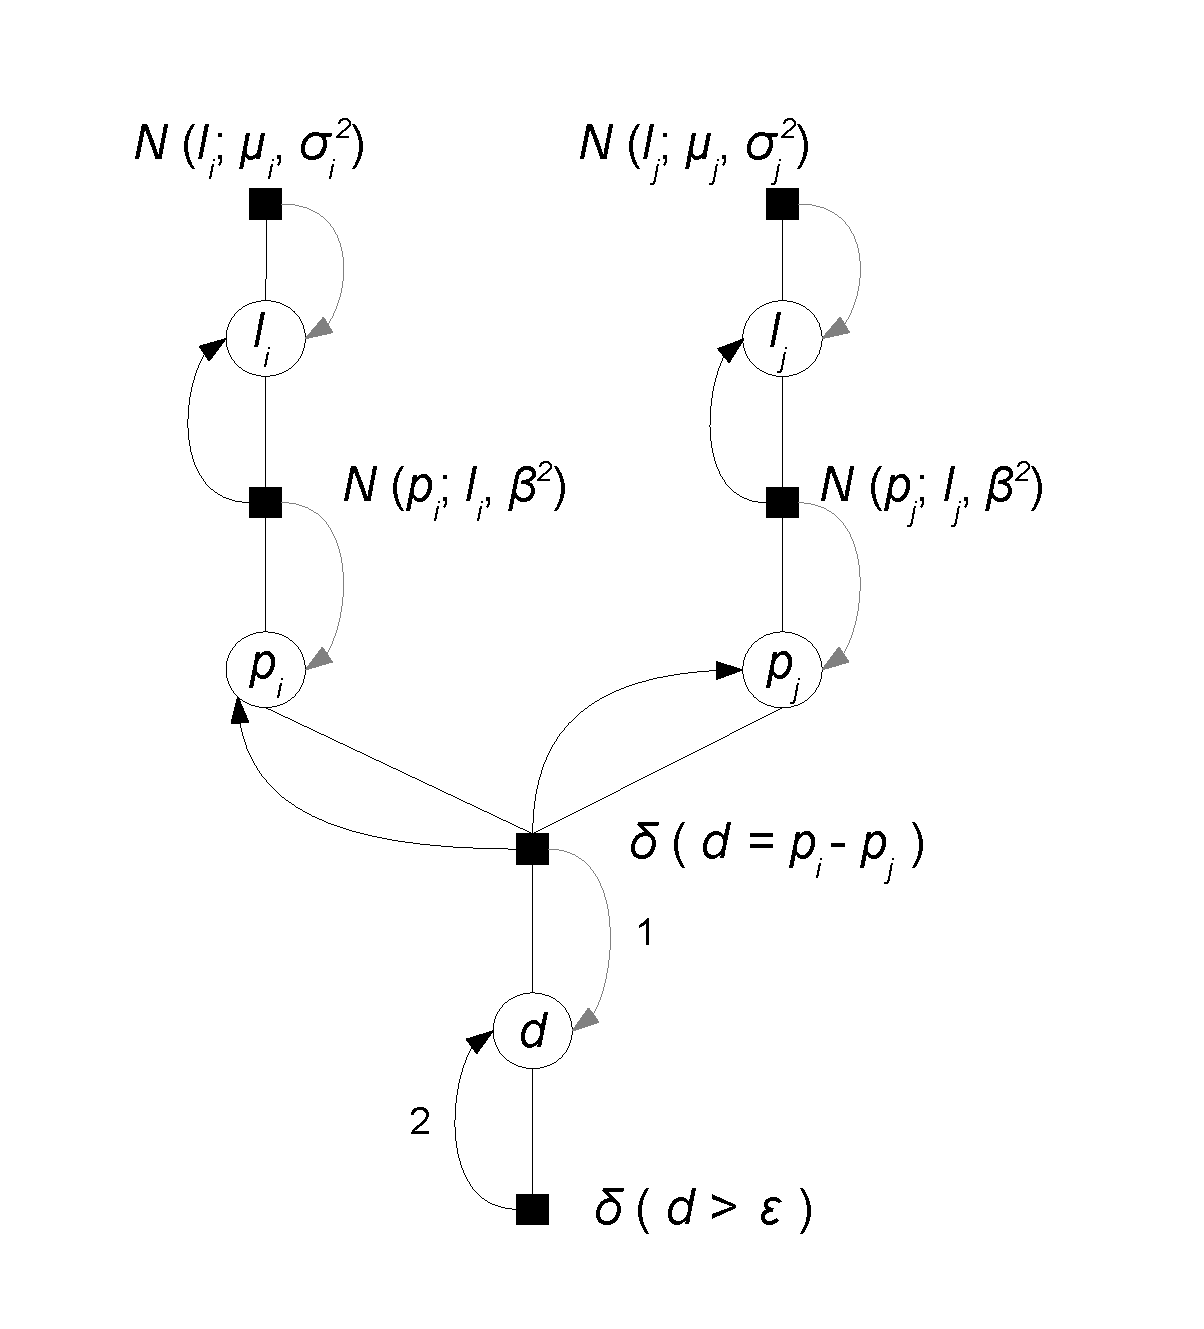
\includegraphics[scale=0.3]{TrueSkill}}
%\centerline{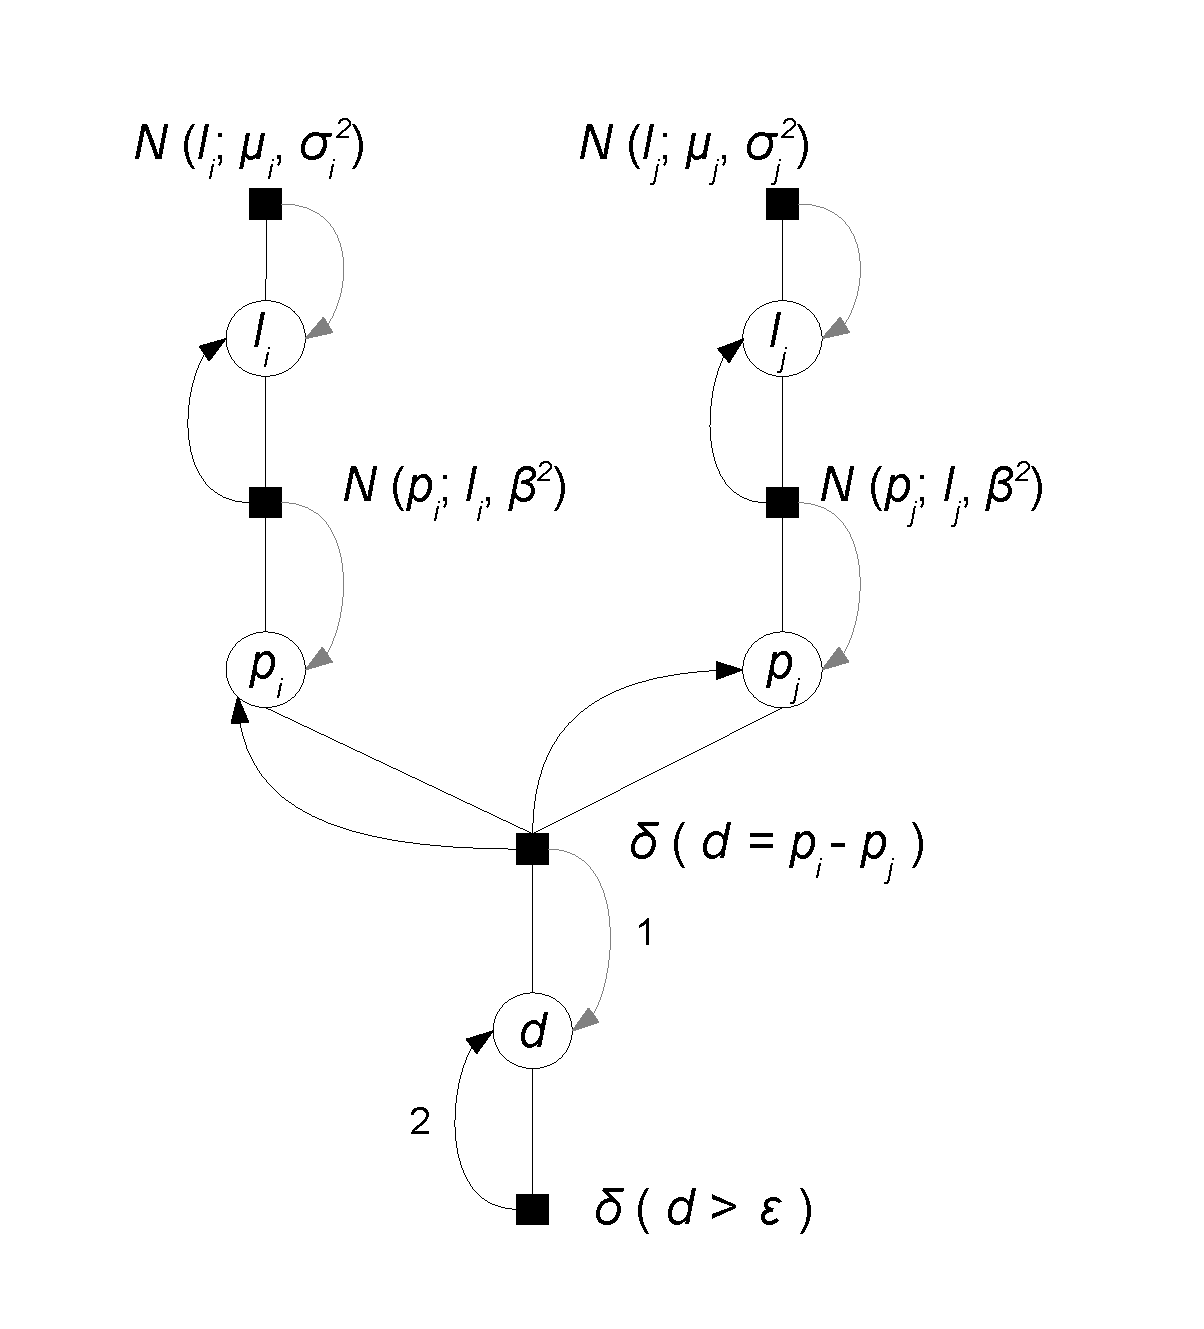
\includegraphics[scale=0.275]{TrueSkill}}
\caption{\small TrueSkill factor graph for a match between two single-player
teams with team i winning.
There are three types of variables: $l_i$
for the skills of all players, $p_i$ for the performances of all
players and $d$ the performance difference. The first row of factors
encode the (product) prior; the product of the remaining factors
characterizes the likelihood for the game outcome team $i$ winning team $j$.
The arrows show the optimal message passing schedule: (1)
messages pass along \emph{gray} arrows from top to bottom, (2) the
marginal over $d$ is updated via message 1 followed by message 2
(which requires moment matching), (3) messages pass from bottom to top
along \emph{black} arrows.}
\label{fig:trueskill}
\vspace{-3mm}
\end{figure}

TrueSkill is an efficient and principled Bayesian skill learning
system.  However, due to its design goals, it discards score
information and does not take into account associated domain knowledge
such as offence/defence skill components.  Next,
we propose extensions of the TrueSkill factor graph and (approximate)
inference algorithms for score-based Bayesian skill learning, which
address these limitations.
